\chapter{Latin Words}
\label{chap:latinwords}

\lipsum[1]



\section{Latin Words with a Table}
\label{sec:latinwords}

The data presented in Fig.~\ref{tab:lanechangeresults} is clearly doctored to agree with what I want it to say.


\begin{table}[htbp] \centering \caption{Cone pairs chosen in the lane change replication test}
\begin{tabular}{rc|cc} 
    GUI&    Run \#  &     Leader&    Follower \\ \hline\hline
    Earth&      1       &       1   &    3 \\
         &      2       &       3   &    4   \\ \hline
    Monolith&   3       &       2   &    3   \\
         &      4       &       5   &    5 \\ \hline   
\end{tabular} \label{tab:lanechangeresults} \end{table}

\lipsum[2]



\subsection{Latin Words \& Some Figures}
\label{sec:latinwordsfigs}

Depicted below in Figs.~\ref{fig:platypus} and \ref{fig:pangolin} are two adorable animals. 

\begin{figure}[ht] \centering
    \begin{minipage}[b]{0.45\linewidth} \centering 
        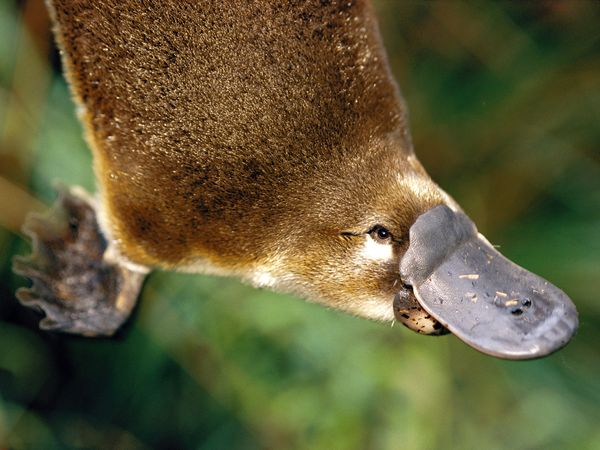
\includegraphics[width=\textwidth]{./figs/a_cute_platypus.jpg}
        \caption{Platypi swim in water often.} \label{fig:platypus}
    \end{minipage}
    \hspace{0.5cm}
    \begin{minipage}[b]{0.45\linewidth} \centering
        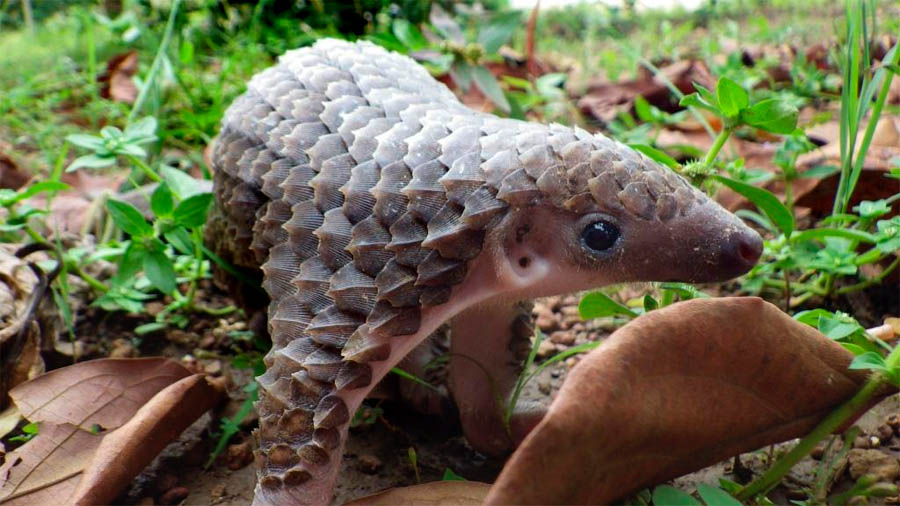
\includegraphics[width=\textwidth]{./figs/an_adorable_pangolin.jpg}
        \caption{The pangolin is not a fuzzy animal.} \label{fig:pangolin}
    \end{minipage}
\end{figure}

To see an animal for which an OS version was named, see Fig.~\ref{fig:quetzal} .

\lipsum[3]